\documentclass{article}
\usepackage{amsmath}
\usepackage{graphicx}
\usepackage{subcaption}
\usepackage[left=2cm,top=2.5cm,right=1.5cm,bottom=2.5cm]{geometry}
\usepackage{tikz}
\usepackage{pgfplots}
\pgfplotsset{compat=1.15}
\usetikzlibrary{external}
\usepgfplotslibrary{external}
\tikzexternalize
\DeclareMathOperator{\I}{I}

\begin{document}
\begin{figure}[!ht]
\begin{center}
\begin{subfigure}{0.45\textwidth}
\centering
\tikzsetnextfilename{group-law-secant}
\begin{tikzpicture}[scale=1.5]
\newcommand{\avar}{-1}
\newcommand{\bvar}{0.7}
\newcommand{\xmax}{1.5}
\newcommand{\excx}{0.00017547}
\newcommand{\xp}{-1}
\newcommand{\xq}{-0.2}
\newcommand{\exc}{1}
\newcommand{\excy}{0.6}

\newcommand{\xmin}{-(-sqrt(27*(\bvar)^2+4*(\avar)^3)/(2*3^(3/2))+\bvar/2)^(1/3)+\avar/(3*(-sqrt(27*(\bvar)^2+4*(\avar)^3)/(2*3^(3/2))+\bvar/2)^(1/3))-\excx}
\newcommand{\ymax}{sqrt((\xmax)^3+\avar*\xmax+\bvar)}
\newcommand{\yp}{sqrt((\xp)^3+\avar*\xp+\bvar)}
\newcommand{\yq}{sqrt((\xq)^3+\avar*\xq+\bvar)}
\newcommand{\slope}{(\yq-\yp)/(\xq-\xp)}
\newcommand{\xr}{(\slope)^2-\xp-\xq}
\newcommand{\yr}{\slope*(\xr-\xp)+\yp}
\draw [smooth,samples=100,domain={\xmin}:\xmax] plot(\x,{sqrt((\x)^3+\avar*\x+\bvar)});
\draw [smooth,samples=100,domain={\xmin}:\xmax] plot(\x,{-sqrt((\x)^3+\avar*\x+\bvar)});
\draw [fill] (\xp,{\yp}) circle (1.5pt);
\draw [above left] (\xp,{\yp}) node {$P$};
\draw [fill] (\xq,{\yq}) circle (1.5pt);
\draw [above right] (\xq,{\yq}) node {$Q$};
\draw ({\xmin-\exc},{\slope*(\xmin-\exc-\xp)+\yp}) -- (\xmax+\exc,{\slope*(\xmax+\exc-\xp)+\yp});
\draw [fill] ({\xr},{\yr}) circle (1.5pt);
\draw [above left] ({\xr},{\yr}) node {$R$};
\draw [->,dash pattern=on 4pt off 4pt] ({\xr},{-\ymax-\excy}) -- ({\xr},{\ymax+\excy});
\draw [above right] ({\xr},{\ymax+\excy}) node {$O$};
\draw [fill] ({\xr},{-(\yr)}) circle (1.5pt);
\draw [below left] ({\xr},{-(\yr)}) node {$P\oplus Q$};
\end{tikzpicture}

\caption{Sum of two distinct points.}
\end{subfigure}
\begin{subfigure}{0.45\textwidth}
\centering
\tikzsetnextfilename{group-law-tangent}
\begin{tikzpicture}[scale=1.5]
\newcommand{\avar}{-1}
\newcommand{\bvar}{0.7}
\newcommand{\xmax}{1.5}
\newcommand{\excx}{0.00017547}
\newcommand{\xp}{-0.5}
\newcommand{\exc}{1}
\newcommand{\excy}{0.6}

\newcommand{\xmin}{-(-sqrt(27*(\bvar)^2+4*(\avar)^3)/(2*3^(3/2))+\bvar/2)^(1/3)+\avar/(3*(-sqrt(27*(\bvar)^2+4*(\avar)^3)/(2*3^(3/2))+\bvar/2)^(1/3))-\excx}
\newcommand{\ymax}{sqrt((\xmax)^3+\avar*\xmax+\bvar)}
\newcommand{\yp}{sqrt((\xp)^3+\avar*\xp+\bvar)}
\newcommand{\slope}{(3*(\xp)^2+\avar)/(2*\yp)}
\newcommand{\xr}{(\slope)^2-2*\xp}
\newcommand{\yr}{\slope*(\xr-\xp)+\yp}
\draw [smooth,samples=100,domain={\xmin}:\xmax] plot(\x,{sqrt((\x)^3+\avar*\x+\bvar)});
\draw [smooth,samples=100,domain={\xmin}:\xmax] plot(\x,{-sqrt((\x)^3+\avar*\x+\bvar)});
\draw [fill] (\xp,{\yp}) circle (1.5pt);
\draw [above left] (\xp,{\yp}) node {$P$};
\draw ({\xmin-\exc},{\slope*(\xmin-\exc-\xp)+\yp}) -- ({\xmax+\exc},{\slope*(\xmax+\exc-\xp)+\yp});
\draw [fill] ({\xr},{\yr}) circle (1.5pt);
\draw [above left] ({\xr},{\yr}) node {$R$};
\draw [->,dash pattern=on 4pt off 4pt] ({\xr},{-\ymax-\excy}) -- ({\xr},{\ymax+\excy});
\draw [above right] ({\xr},{\ymax+\excy}) node {$O$};
\draw [fill] ({\xr},{-(\yr)}) circle (1.5pt);
\draw [below left] ({\xr},{-(\yr)}) node {$P\oplus P$};
\draw [fill] ({\xmin},0) circle (1.5pt);
\draw [left] ({\xmin},0) node {$T$};
\draw [->,dash pattern=on 4pt off 4pt] ({\xmin},{-\ymax-\excy}) -- ({\xmin},{\ymax+\excy});
\draw [above right] ({\xmin},{\ymax+\excy}) node {$O$};
\draw [below right] ({\xmin},{-(\yr)-\exc/2}) node {$T\oplus T=O$};
\end{tikzpicture}

\caption{Sum of a point with itself.}
\end{subfigure}
\caption{Illustration of the group law of elliptic curves. Modified from: [Sil09, Figure~3.3].}
\end{center}
\end{figure}

\begin{figure}[!ht]
\begin{center}
\begin{subfigure}{\textwidth}
\centering
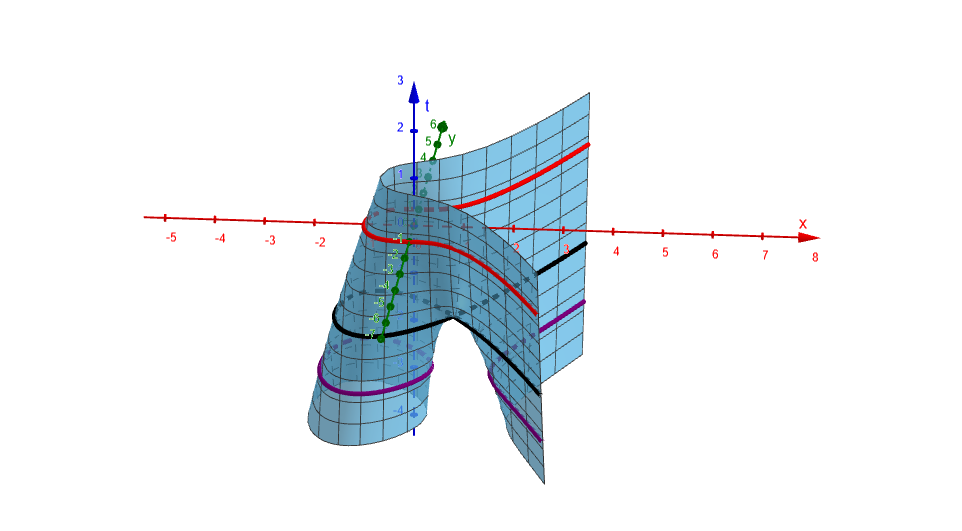
\includegraphics[scale=0.5]{elliptic-surface.png}
\caption{Elliptic surface $y^2=x^3+tx+1$.}
\end{subfigure}
\vspace{10mm}

\begin{subfigure}{0.3\textwidth}
\centering
\tikzsetnextfilename{elliptic-fibres-neg}
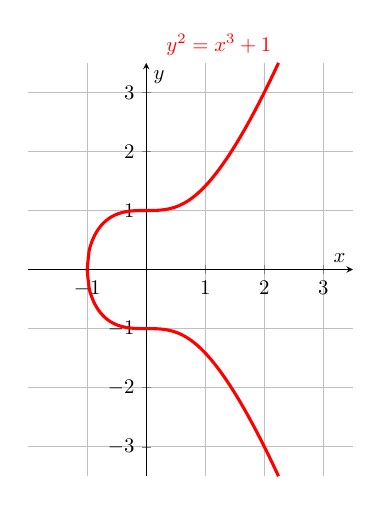
\begin{tikzpicture}[scale=0.75]
\newcommand{\avar}{0}
\newcommand{\bvar}{1}
\newcommand{\ymax}{3.5}
%\newcommand{\excx}{0.00008392}
\newcommand{\excx}{0}
\newcommand{\lw}{1.5}

\newcommand{\xmax}{2.24070237327858}
\newcommand{\xmin}{-1}
\begin{axis}
[grid=both,x=1cm,y=1cm,ymin=-3.5,ymax=3.5,xmax=3.5,xmin=-2,xtick={-1,...,3},ytick={-3,...,3},axis lines=middle,xlabel=$x$,ylabel=$y$,clip=false]
\draw [line width=\lw pt,smooth,samples=100,domain=\xmin-\excx:\xmax,color=red] plot(\x,{sqrt((\x)^3+\avar*\x+\bvar)});
\draw [line width=\lw pt,smooth,samples=100,domain=\xmin-\excx:\xmax,color=red] plot(\x,{-sqrt((\x)^3+\avar*\x+\bvar)});
\draw [above left,color=red] ({\xmax},\ymax) node {$y^2=x^3+1$};
\end{axis}
\end{tikzpicture}

\caption{Fibre at $t=0$.}
\end{subfigure}
\begin{subfigure}{0.3\textwidth}
\centering
\tikzsetnextfilename{elliptic-fibres-zero}
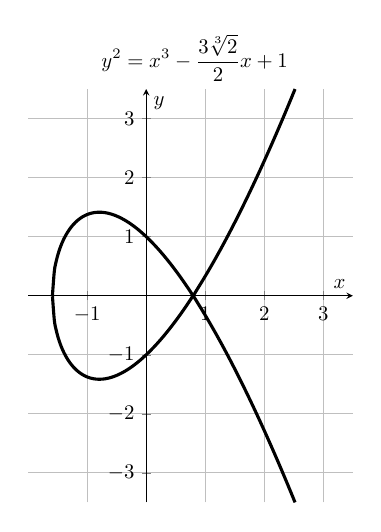
\begin{tikzpicture}[scale=0.75]
\newcommand{\avar}{-3/4^(1/3)}
\newcommand{\bvar}{1}
\newcommand{\ymax}{3.5}
%\newcommand{\exc}{0.006798}
\newcommand{\exc}{0.003579}
%\newcommand{\glum}{0.02}
\newcommand{\glum}{0.01}
%\newcommand{\glun}{0.15}
\newcommand{\glun}{0.2}
\newcommand{\lw}{1.5}

\newcommand{\xmax}{2.52055306100453}
\newcommand{\xmin}{-1.58740105196820}
\newcommand{\xnode}{0.793700525984100}
\begin{axis}
[grid=both,x=1cm,y=1cm,ymin=-3.5,ymax=3.5,xmax=3.5,xmin=-2,xtick={-1,...,3},ytick={-3,...,3},axis lines=middle,xlabel=$x$,ylabel=$y$,clip=false]
\draw [line width=\lw pt,smooth,samples=75,domain=\xmin:\xnode-\exc] plot(\x,{sqrt((\x)^3+\avar*\x+\bvar)});
\draw [line width=\lw pt,smooth,domain=\xnode+\exc:\xmax] plot(\x,{sqrt((\x)^3+\avar*\x+\bvar)});
\draw [line width=\lw pt,smooth,samples=75,domain=\xmin:\xnode-\exc] plot(\x,{-sqrt((\x)^3+\avar*\x+\bvar)});
\draw [line width=\lw pt,smooth,domain=\xnode+\exc:\xmax] plot(\x,{-sqrt((\x)^3+\avar*\x+\bvar)});
\draw [above left] ({\xmax},\ymax) node {$\displaystyle{y^2=x^3-\frac{3\sqrt[3]{2}}{2}x+1}$};
\draw [line width=\lw pt] ({\xmin},-\glum) -- ({\xmin},\glum);
\draw [fill] ({\xnode},0) circle (\glun pt);
\end{axis}
\end{tikzpicture}

\caption{Fibre at $t=-\frac{3\sqrt[3]{2}}{2}$.}
\end{subfigure}
\begin{subfigure}{0.3\textwidth}
\centering
\tikzsetnextfilename{elliptic-fibres-pos}
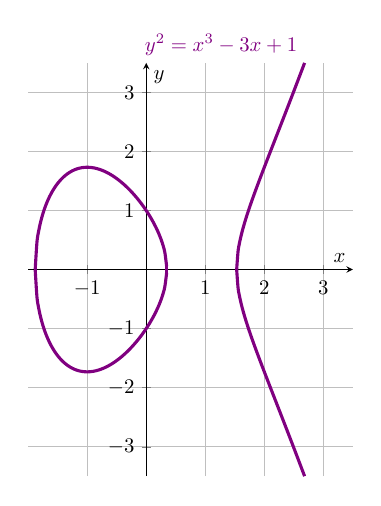
\begin{tikzpicture}[scale=0.75]
\newcommand{\avar}{-3}
\newcommand{\bvar}{1}
\newcommand{\ymax}{3.5}
%\newcommand{\exc}{0.000007630}
\newcommand{\exc}{0}
\newcommand{\glui}{0.009}
\newcommand{\gluii}{0.055}
\newcommand{\gluiii}{0.01}
\newcommand{\lw}{1.5}

\newcommand{\xmax}{2.68221750204240}
\newcommand{\xmin}{-1.87938524157182}
\newcommand{\xii}{0.347296355333861}
\newcommand{\xiii}{1.53208888623796}
\begin{axis}
[grid=both,x=1cm,y=1cm,ymin=-3.5,ymax=3.5,xmax=3.5,xmin=-2,xtick={-1,...,3},ytick={-3,...,3},axis lines=middle,xlabel=$x$,ylabel=$y$,clip=false]
\draw [line width=\lw pt,smooth,samples=75,domain=\xmin:\xii,color=violet] plot(\x,{sqrt((\x)^3+\avar*\x+\bvar)});
\draw [line width=\lw pt,smooth,samples=50,domain=\xiii+\exc:\xmax,color=violet] plot(\x,{sqrt((\x)^3+\avar*\x+\bvar)});
\draw [line width=\lw pt,smooth,samples=75,domain=\xmin:\xii,color=violet] plot(\x,{-sqrt((\x)^3+\avar*\x+\bvar)});
\draw [line width=\lw pt,smooth,samples=50,domain=\xiii+\exc:\xmax,color=violet] plot(\x,{-sqrt((\x)^3+\avar*\x+\bvar)});
\draw [above left,color=violet] ({\xmax},\ymax) node {$y^2=x^3-3x+1$};
\draw [line width=\lw pt,color=violet] ({\xmin},-\glui) -- ({\xmin},\glui);
\draw [line width=\lw pt,color=violet] ({\xii},-\gluii) -- ({\xii},\gluii);
\draw [line width=\lw pt,color=violet] ({\xiii},-\gluiii) -- ({\xiii},\gluiii);
\end{axis}
\end{tikzpicture}

\caption{Fibre at $t=-3$.}
\end{subfigure}
\caption{Representation in the real space of the elliptic surface $y^2=x^3+tx+1$ with its fibres at $t=0$ ($\Delta=-432$), $t=-\frac{3\sqrt[3]{2}}{2}$ ($\Delta=0$), $t=-3$ ($\Delta=1296$). The fibre at $t=a$ is obtained geometrically by intersecting the surface with the horizontal plane $t=a$.}
\end{center}
\end{figure}

\begin{figure}[!ht]
\begin{center}
\begin{subfigure}{0.45\textwidth}
\centering
\tikzsetnextfilename{singular-fibres-1}
\begin{tikzpicture}
\newcommand{\ymax}{1.5}
\newcommand{\xhead}{1.5}
\newcommand{\exc}{0.5}

\newcommand{\xmax}{(sqrt(((\ymax+\exc)/\xhead)^2*(27*((\ymax+\exc)/\xhead)^2-4))/(2*3^(3/2))+((\ymax+\exc)/\xhead)^2/2+(-1)/27)^(1/3)+1/(9*(sqrt(((\ymax+\exc)/\xhead)^2*(27*((\ymax+\exc)/\xhead)^2-4))/(2*3^(3/2))+((\ymax+\exc)/\xhead)^2/2+(-1)/27)^(1/3))+(-1)/3}
\draw [smooth,samples=75,domain=-1:0] plot(\xhead*\x,{\xhead*sqrt((\x)^(2)+(\x)^(3))});
\draw [smooth,domain=0:{\xmax}] plot(\xhead*\x,{\xhead*sqrt((\x)^(2)+(\x)^(3))});
\draw [smooth,samples=75,domain=-1:0] plot(\xhead*\x,{-\xhead*sqrt((\x)^(2)+(\x)^(3))});
\draw [smooth,domain=0:{\xmax}] plot(\xhead*\x,{-\xhead*sqrt((\x)^(2)+(\x)^(3))});
\end{tikzpicture}

\caption{Singular fibre of type $\I_1$.}
\end{subfigure}
\begin{subfigure}{0.45\textwidth}
\centering
\tikzsetnextfilename{singular-fibres-2}
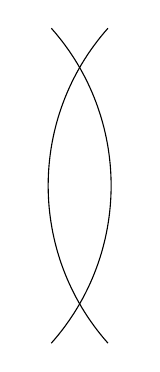
\begin{tikzpicture}
\newcommand{\ymax}{1.5}
\newcommand{\width}{0.4}
\newcommand{\exc}{0.5}

\draw ({(\ymax)^2/(2*\width)-\width/2-sqrt(((\ymax)^2/(2*\width)+\width/2)^2-(\ymax+\exc)^2)},\ymax+\exc) arc ({180-asin((\ymax+\exc)/((\ymax)^2/(2*\width)+\width/2))}:{180+asin((\ymax+\exc)/((\ymax)^2/(2*\width)+\width/2))}:{(\ymax)^2/(2*\width)+\width/2});
\draw ({-((\ymax)^2/(2*\width)-\width/2-sqrt(((\ymax)^2/(2*\width)+\width/2)^2-(\ymax+\exc)^2))},\ymax+\exc) arc ({asin((\ymax+\exc)/((\ymax)^2/(2*\width)+\width/2))}:{-asin((\ymax+\exc)/((\ymax)^2/(2*\width)+\width/2))}:{(\ymax)^2/(2*\width)+\width/2});
\end{tikzpicture}

\caption{Singular fibre of type $\I_2$.}
\end{subfigure}
\vspace{20mm}

\begin{subfigure}{0.45\textwidth}
\centering
\tikzsetnextfilename{singular-fibres-3}
\begin{tikzpicture}
\newcommand{\ymax}{1.5}
\newcommand{\exc}{0.5}

\draw ({-2*sqrt(3)/3*\ymax-sqrt(3)/3*\exc},{-\ymax-\exc}) -- ({sqrt(3)/3*\exc},{\ymax+\exc});
\draw ({-sqrt(3)/3*\exc},{\ymax+\exc}) -- ({2*sqrt(3)/3*\ymax+sqrt(3)/3*\exc},{-\ymax-\exc});
\draw ({2*sqrt(3)/3*\ymax+2*sqrt(3)/3*\exc},{-\ymax}) -- ({-2*sqrt(3)/3*\ymax-2*sqrt(3)/3*\exc},{-\ymax});
\end{tikzpicture}

\caption{Singular fibre of type $\I_3$.}
\end{subfigure}
\begin{subfigure}{0.45\textwidth}
\centering
\tikzsetnextfilename{singular-fibres-4}
\begin{tikzpicture}
\newcommand{\ymax}{1.5}
\newcommand{\exc}{0.5}

\draw ({-sqrt(3)/3*\ymax+sqrt(3)/3*\exc},{-\ymax-\exc}) -- ({-2*sqrt(3)/3*\ymax-sqrt(3)/3*\exc},\exc);
\draw ({-2*sqrt(3)/3*\ymax-sqrt(3)/3*\exc},-\exc) -- ({-sqrt(3)/3*\ymax+sqrt(3)/3*\exc},{\ymax+\exc});
\draw ({sqrt(3)/3*\ymax-sqrt(3)/3*\exc},{\ymax+\exc}) -- ({2*sqrt(3)/3*\ymax+sqrt(3)/3*\exc},-\exc);
\draw ({2*sqrt(3)/3*\ymax+sqrt(3)/3*\exc},\exc) -- ({sqrt(3)/3*\ymax-sqrt(3)/3*\exc},{-\ymax-\exc});
\draw (0,\ymax) node {$\cdots$};
\draw (0,-\ymax) node {$\cdots$};
\end{tikzpicture}

\caption{Singular fibre of type $\I_4$.}
\end{subfigure}
\caption{Illustration of the singular fibres of type $\I_m$ in an elliptic surface. Modified from: [SS19, Figure~5.1].}
\end{center}
\end{figure}
\end{document}
